% THIS TEMPLATE IS A WORK IN PROGRESS

\documentclass[polish, a4paper]{article}
\usepackage[a4paper,left=3cm,right=3cm,top=3cm,bottom=1.5cm]{geometry}
\usepackage[T1]{fontenc}
\usepackage[polish]{babel}
\usepackage[utf8]{inputenc}
\usepackage{hyperref}
\usepackage{fancyhdr}
\usepackage{float}
\usepackage{graphicx}
\usepackage{titling}
\usepackage{caption}
\usepackage{pgfplots}
\usepackage{pgfplotstable}
\usepackage{filecontents}
\usepackage{csvsimple}
\usepackage{textcomp}
\usepackage{gensymb}
%\usepackage{siunitx}
\graphicspath{ {./} }
\pagestyle{fancy}

\setlength{\droptitle}{-1in}

%\lhead{\includegraphics[width=0.2\textwidth]{nyush-logo.pdf}}

  \lhead{Maciej Kaszkowiak}
  \chead{Ćwiczenie 324}
  \rhead{Lab 4,
  151856}


%%%% PROJECT TITLE
\title{Badanie właściwości dielektrycznych ciał stałych\\
        \Large \emph{Ćwiczenie nr 324 z działu Optyka}}

%%%% NAMES OF ALL THE STUDENTS INVOLVED (first-name last-name)
\author{Maciej Kaszkowiak, Lab 4, 151856}

\date{\vspace{-5ex}} %NO DATE


\begin{document}
\maketitle
%\thispagestyle{titlepage}

\section{Cel ćwiczenia}
Przeprowadzone ćwiczenie ma dwa główne cele:
\begin{enumerate}
\item{Wyznaczenie kąta Brewstera oraz współczynnika załamania światła badanego ośrodka. }
\item{Praktyczne i teoretyczne sprawdzenie zależności amplitudowych współczynników odbicia od kąta padania światła.}
\end{enumerate}
\section{Wstęp teoretyczny}

Światło jest falą elektromagnetyczną, czyli rozchodzącymi się w przestrzeni zmiennymi polami elektrycznym i magnetycznym. Przy stosowaniu światła spolaryzowanego liniowo zauważono następujące zależności: przy prostopadłym do płaszczyzny padania wektorze pola elektrycznego fali padającej natężenie światła odbitego rośnie monotonicznie wraz ze wzrostem kąta padania, a przy równoległym do płaszczyzny padania wektorze pola elektrycznego fali padającej natężenie światła w funkcji kąta padania najpierw maleje, dochodząc do wartości zero dla tak zwanego kąta Brewstera, a następnie rośnie. Zgodnie z prawem Snelliusa, stosunek sinusów kąta padania $\alpha$ i kąta załamania $\beta$ jest dla danej pary ośrodków stały, równy stosunkowi bezwzględnych współczynników załamania światła obu ośrodków $\frac{n_2}{n_1}$.

Ze względu na fakt, że promień padający znajduje się w ośrodku składającym się z powietrza ($n_1 \approx 1$) możemy przyjąć, że:

\begin{equation}
\frac{\sin \alpha}{\sin \beta} = n
\end{equation}

gdzie n to bezwzględny współczynnik załamania światła dielektryka. Na potrzeby doświadczenia będziemy próbowali wyznaczyć współczynnik załamania światła dla badanego pryzmatu.

\section{Przebieg ćwiczenia}

\begin{enumerate}
\item{Włączyliśmy zasilanie lasera, miernik napięcia oraz wzmacniacz, a następnie ustawiliśmy położenie na skali rotatora na 0. Ustawienie to odpowiada drganiom wektora elektrycznego prostopadłym do płaszczyzny padania. Odczekaliśmy kilka
minut w celu dostatecznego wygrzania aparatury.}
\item{Zdjęliśmy pryzmat ze stoliczka, a następnie, ustawiając obrotowe ramię z detektorem wzdłuż promienia laserowego, zmierzyliśmy wartość $U_0$.}
\item{Położyliśmy pryzmat na stoliczku i obróciliśmy stoliczek tak, aby kąt padania wynosił 10\degree. Zmierzyliśmy wartość napięcia U dla kątów padania w zakresie od 10\degree \; do 85\degree \; ze skokiem co 5\degree.}
\item{Za pomocą rotatora skręciliśmy płaszczyznę polaryzacji światła o kąt 90\degree. Powtórzyliśmy pomiary w zakresie od 10\degree \; do 85\textdegree \; ze skokiem co 5\degree. W pobliżu kąta, dla którego występuje wygaszenie wiązki odbitej, zagęściliśmy pomiary wykonując je co 1\degree.}
\end{enumerate}

\begin{figure}[H]
\centering
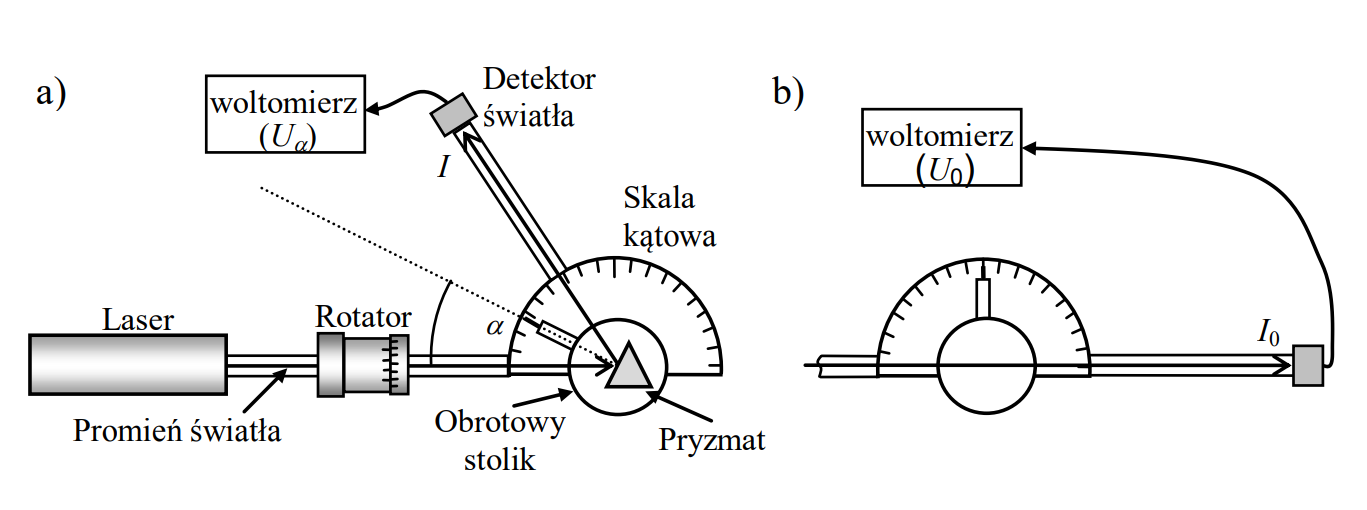
\includegraphics[width=\textwidth]{woltomierz.png}
\caption{Schemat układu pomiarowego służącego do wyznaczenia współczynników odbicia
światła: a) pomiar natężenia światła laserowego odbitego od powierzchni dielektryka, b)
bezpośredni pomiar natężenia światła laserowego}
\end{figure}

\section{Wyniki pomiarów}


Wartość napięcia początkowego lasera $U_0$ wynosi $1,395 V$.

Znając $U_0$ oraz $U_\alpha$ obliczyłem bezwzględne wartości współczynników Fresnela $| \xi_\alpha |$ dla poszczególnych kątów padania, korzystając ze wzoru:

\begin{equation}
| \xi_\alpha | = \sqrt{R_\alpha} = \sqrt{\frac{U_\alpha}{U_0}}
\end{equation}

gdzie $R_\alpha$ to współczynnik odbicia światła dla kąta $\alpha$.

\begin{table}[H]
    \centering
    \begin{tabular}{|l|l|l|}
    \hline
        Kąt [stopnie] & Napięcie [V] & Współczynnik Fresnela \\ \hline
        10 & 0,041 & 0,171 \\ \hline
        15 & 0,033 & 0,154 \\ \hline
        20 & 0,031 & 0,149 \\ \hline
        25 & 0,029 & 0,144 \\ \hline
        30 & 0,025 & 0,134 \\ \hline
        35 & 0,023 & 0,128 \\ \hline
        40 & 0,019 & 0,117 \\ \hline
        45 & 0,014 & 0,100 \\ \hline
        50 & 0,012 & 0,093 \\ \hline
        51 & 0,010 & 0,085 \\ \hline
        52 & 0,011 & 0,089 \\ \hline
        53 & 0,011 & 0,089 \\ \hline
        54 & 0,011 & 0,089 \\ \hline
        55 & 0,011 & 0,089 \\ \hline
        60 & 0,017 & 0,110 \\ \hline
        65 & 0,027 & 0,139 \\ \hline
        70 & 0,078 & 0,236 \\ \hline
        75 & 0,171 & 0,350 \\ \hline
        80 & 0,352 & 0,502 \\ \hline
        85 & 0,252 & 0,425 \\ \hline
    \end{tabular}
    \caption{Pomiar napięcia w zależności od kąta padania lasera na pryzmat przy kącie polaryzacji 90 stopni}
\end{table}

\begin{table}[H]
    \centering
    \begin{tabular}{|l|l|l|}
    \hline
        Kąt [stopnie] & Napięcie [V] & Współczynnik Fresnela \\ \hline
        10 & 0,037 & 0,163 \\ \hline
        15 & 0,038 & 0,165 \\ \hline
        20 & 0,039 & 0,167 \\ \hline
        25 & 0,043 & 0,176 \\ \hline
        30 & 0,047 & 0,184 \\ \hline
        35 & 0,054 & 0,197 \\ \hline
        40 & 0,061 & 0,209 \\ \hline
        45 & 0,070 & 0,224 \\ \hline
        50 & 0,091 & 0,255 \\ \hline
        55 & 0,117 & 0,290 \\ \hline
        60 & 0,158 & 0,337 \\ \hline
        65 & 0,209 & 0,387 \\ \hline
        70 & 0,300 & 0,464 \\ \hline
        75 & 0,390 & 0,529 \\ \hline
        80 & 0,528 & 0,615 \\ \hline
        85 & 0,260 & 0,432 \\ \hline
    \end{tabular}
    \caption{Pomiar napięcia w zależności od kąta padania lasera na pryzmat przy kącie polaryzacji 0 stopni}
\end{table}

\section{Opracowanie wyników}

\begin{figure}[H]
\centering
\begin{tikzpicture}
\begin{axis}[
    width=\textwidth, height=0.8\textwidth,
    grid=major,
    xlabel={Kąt (stopnie)},
    ylabel={Bewzględny współczynnik Fresnela},
    ymin=0, ymax=0.7,
    legend style={at={(0.05,0.95)},anchor=north west}
]
\addplot+[
    smooth,
    orange
] table[
    x = degree, col sep=comma,
    y = fresnel
] {polaryzacja0.csv};
\addlegendentry{Pomiar $f(\alpha)=|\xi_\alpha^\bot |$}

\addplot+[
    smooth,
    blue
] table[
    x = degree, col sep=comma,
    y = fresnel
] {polaryzacja90.csv};
\addlegendentry{Pomiar $f(\alpha)=|\xi_\alpha^\parallel |$}
\end{axis}
\end{tikzpicture}
\caption{Wyznaczone doświadczalnie wartości bezwzględnych współczynników Fresnela w zależności od kąta padania lasera.}
\end{figure}

Z wykresu $f(\alpha)=|\xi_\alpha^\parallel |$ możemy odczytać kąt Brewstera wynoszący 51\textdegree, znany również jako kąt całkowitej polaryzacji.

Znając kąt Brewstera możemy wyznaczyć współczynnik załamania światła $n$ dla materiału, z którego wykonany jest pryzmat:

\begin{equation}
    n = \tan \alpha_B = \tan 51 \degree \approx 1,23
\end{equation}

Znając współczynnik załamania światła pryzmatu możemy wyliczyć teoretyczne wartości współczynnika Fresnela korzystając z następujących wzorów:

\begin{equation}
    |\xi_\alpha^\parallel | = \left\| \frac{
        n^2 \cos \alpha - \sqrt{n^2 - \sin^2 \alpha}    
    }{
        n^2 \cos \alpha + \sqrt{n^2 - \sin^2 \alpha}    
    } \right\|
\end{equation}

\begin{equation}
    |\xi_\alpha^\bot | = \left\| \frac{
        (\sqrt{n^2 - \sin^2 \alpha} - \cos \alpha)^2
    }{
        n^2 - 1
    } \right\|
\end{equation}


\begin{table}[H]
    \centering
    \begin{tabular}{|l|l|l|}
    \hline
        & Współczynnik Fresnela & Współczynnik Fresnela \\ 
        \bfseries Kąt~[stopnie] & \bfseries Polaryzacja~prostopadła & \bfseries Polaryzacja~równoległa
        \csvreader[]{teoria.csv}{}
        {\\ \hline \csvcoli & \csvcolii & \csvcoliii }
        \\ \hline
    \end{tabular}
    
    \caption{Współczynnik Fresnela w zależności od kąta padania lasera oraz kątu polaryzacji.}
\end{table}

Ewentualne drobne rozbieżności wynikają z zaokrąglenia tangensa kąta 51 stopni do dwóch miejsc po przecinku.

\begin{figure}[H]
\centering
\begin{tikzpicture}
\begin{axis}[
    width=\textwidth, height=0.8\textwidth,
    grid=major,
    xlabel={Kąt (stopnie)},
    ylabel={Bewzględny współczynnik Fresnela},
    ymin=0, ymax=0.9,
    legend style={at={(0.05,0.95)},anchor=north west}
]
\addplot+[
    smooth,
    orange
] table[
    x = degree, col sep=comma,
    y = fresnel0
] {teoria.csv};
\addlegendentry{Teoretyczne $f(\alpha)=|\xi_\alpha^\bot |$}

\addplot+[
    smooth,
    blue
] table[
    x = degree, col sep=comma,
    y = fresnel90
] {teoria.csv};
\addlegendentry{Teoretyczne $f(\alpha)=|\xi_\alpha^\parallel |$}
\end{axis}
\end{tikzpicture}
\caption{Teoretyczne wartości bezwzględnych współczynników Fresnela w zależności od kąta padania lasera.}
\end{figure}

\begin{figure}[H]
\centering
\begin{tikzpicture}
\begin{axis}[
    width=\textwidth, height=0.8\textwidth,
    grid=major,
    xlabel={Kąt (stopnie)},
    ylabel={Bewzględny współczynnik Fresnela},
    ymin=0, ymax=0.9,
    legend style={at={(0.05,0.95)},anchor=north west}
]
\addplot+[
    smooth,
    orange,
    mark=triangle
] table[
    x = degree, col sep=comma,
    y = fresnel0
] {teoria.csv};
\addlegendentry{Teoretyczne $f(\alpha)=|\xi_\alpha^\bot |$}

\addplot+[
    smooth,
    blue,
    mark=triangle
] table[
    x = degree, col sep=comma,
    y = fresnel90
] {teoria.csv};
\addlegendentry{Teoretyczne $f(\alpha)=|\xi_\alpha^\parallel |$}

\addplot+[
    smooth,
    orange,
    mark=o
] table[
    x = degree, col sep=comma,
    y = fresnel
] {polaryzacja0.csv};
\addlegendentry{Pomiar $f(\alpha)=|\xi_\alpha^\bot |$}

\addplot+[
    smooth,
    blue,
    mark=o
] table[
    x = degree, col sep=comma,
    y = fresnel
] {polaryzacja90.csv};
\addlegendentry{Pomiar $f(\alpha)=|\xi_\alpha^\parallel |$}
\end{axis}
\end{tikzpicture}
\caption{Porównanie pomiarów i teoretycznych wartości bezwzględnych współczynników Fresnela w zależności od kąta padania lasera.}
\end{figure}

Można zauważyć, że teoretyczna wartość współczynnika Fresnela dla lasera z równoległym wektorem pola elektrycznego (dla $\alpha_B = 51\degree$) wynosi 0, gdzie zmierzona wartość wynosi 0,085. Spowodowane jest to dodatkowym źródłem światła w pomieszczeniu, w którym wykonywane były pomiary. Rozproszone światło w pracowni z lampek padało na czujnik, zwiększając wartość zmierzonego napięcia. Na pomiary wpłynęła również niedoskonałość miernika napięcia oraz czujki światła, a także możliwy błąd manualny spowodowany niedoskonałym ustawieniem czujki. 

Dla kąta 85\textdegree \; wartość napięcia rzeczywistego znacząco spadła odbiegając od wartości teoretycznej dla obu kątów polaryzacji, przyjmując identyczną wartość w obu przypadkach. Jest to błędny pomiar, nie potrafiłem natomiast ustalić jego dokładnej przyczyny. Rozpatrywaną przeze mnie możliwością jest niedoskonałość pryzmatu lub błąd przy przepisywaniu wyników. Poza punktem 85 stopni kształt krzywej pokrywa się z krzywą teoretyzcną. 
\section{Wnioski}

Za pomocą doświadczenia wyznaczyłem kąt Brewstera ($\alpha_B \approx 51\degree$) i współczynnik załamania światła ($n \approx 1,23$) dla badanego pryzmatu. Wyznaczyłem bezwzględne współczynniki Fresnela dla danych kątów padania lasera oraz kątów polaryzacji oraz zestawiłem je z pomiarami. Pomiary odbiegają od teoretycznych wartości ze względu na wcześniej wymienione błędy pomiarowe oraz nieidealne warunki eksperymentu, mimo tego możemy zaobserwować charakterystyczny kształt krzywych. Doświadczenie tym samym pokrywa się z teoretycznymi założeniami.


\section{Bibliografia}

\begin{enumerate}
    \item {\emph{Badanie zjawiska odbicia światła od powierzchni
dielektryka} (Krzysztof Łapsa)}
    \item {\emph{Optyka. Ćwiczenie: 324. Badanie zjawiska odbicia światła od powierzchni dielektryka.} (Krzysztof Łapsa) – film na platformie Youtube}
\end{enumerate}


\end{document}
